\documentclass[a4paper,10pt]{article}
\usepackage[utf8]{inputenc}
\usepackage{ngerman}
\usepackage{eurosym}
\usepackage{algorithm2e}
\usepackage{ stmaryrd }
\usepackage{enumerate}
\usepackage{tikz}
\usetikzlibrary{trees,automata,arrows,shapes}
\usepackage{graphicx}
\usepackage{listings}
\usepackage{xcolor}
\usepackage{amsmath, amsthm}
\usepackage{listings}
\usepackage{amsfonts, amssymb}
\usepackage{algorithm2e}
\usepackage{textcomp}
\usepackage{bussproofs}
\usepackage{rotating}
\usepackage{caption}
\usepackage{listings}% http://ctan.org/pkg/listings
\lstset{
  basicstyle=\ttfamily,
  mathescape
}
\renewcommand*{\proofname}{Beweis}

%opening
\title{}
\author{}

\begin{document}
\noindent Thomas Stüber (3750920) \hfill Tübingen, den  21. Oktober 2017\\
\noindent Benjamin Coban () \\
\begin{center}
\Large Übungen zur Vorlesung  \\ ``SAT-Solving und Anwendungen'' \\
\vspace*{2mm}
\large (Abgabe 2) \\
\vspace*{2mm}
\end{center}

\noindent\textbf{Aufgabe 3.1}\\\smallskip
\begin{enumerate}
\item Im folgenden der Ablauf des Algorithmus bis zum ersten Konflikt:
\begin{center}
\begin{tabular}{|c|c|c|c|}
\hline 
\rule[-1ex]{0pt}{2.5ex} Level & Variable & Wert & Grund \\ 
\hline 
\rule[-1ex]{0pt}{2.5ex} 1 & u & $\top$ & decision \\ 
\hline 
\rule[-1ex]{0pt}{2.5ex} 2 & v & $\top$ & decision \\ 
\hline 
\rule[-1ex]{0pt}{2.5ex}  & w & $\top$ & $\{\neg u, \neg v, w\}$ \\ 
\hline 
\rule[-1ex]{0pt}{2.5ex}  & p & $\top$ & $\{\neg u, \neg w, p\}$ \\ 
\hline 
\rule[-1ex]{0pt}{2.5ex}  & z & $\bot$ & $\{\neg u, \neg v, \neg w, \neg z\}$ \\ 
\hline 
\rule[-1ex]{0pt}{2.5ex} 3 & x & $\top$ & decision \\ 
\hline 
\rule[-1ex]{0pt}{2.5ex}  & y & $\bot$ & $\{\neg p, \neg x, \neg y\}$ \\ 
\hline 
\rule[-1ex]{0pt}{2.5ex}  & t & $\top$ & $\{\neg x, y, t\}$ \\ 
\hline 
\rule[-1ex]{0pt}{2.5ex}  & t & $\bot$ & $\{\neg t, \neg w, y\}$ \\ 
\hline 
\end{tabular}
\end{center}
Die Klausel $\{\neg x, y, t\}$ erzwingt $t$ auf wahr zu setzen, während $\{\neg t, \neg w, y\}$ erzwingt $t$ auf falsch zu setzen. Der Implikationsgraph in dieser Konfliktsituation sei im folgenden dargestellt:
\begin{center}
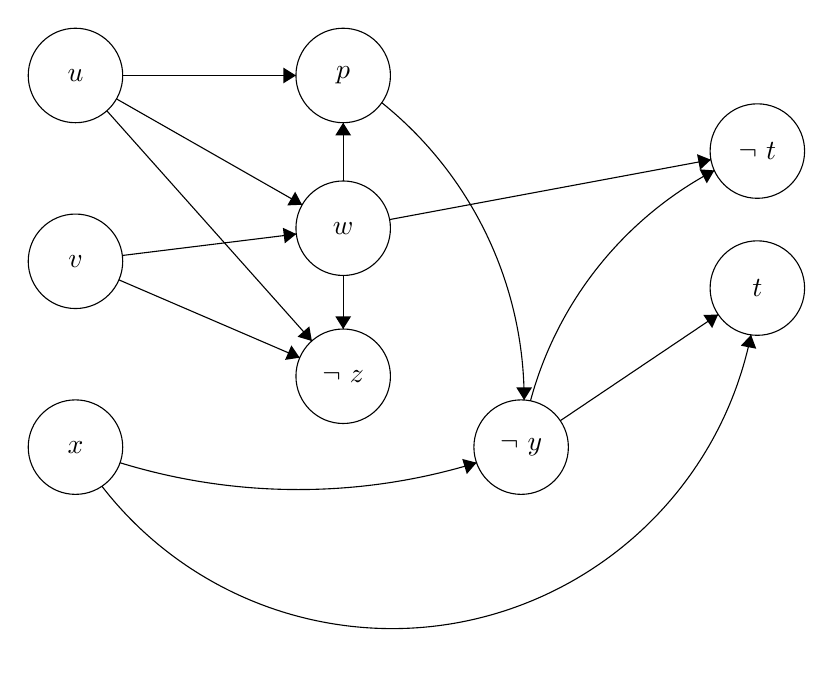
\begin{tikzpicture}[scale=0.2]
\tikzstyle{every node}+=[inner sep=0pt]
\draw [black] (10.2,-9.8) circle (3);
\draw (10.2,-9.8) node {$u$};
\draw [black] (10.2,-21.6) circle (3);
\draw (10.2,-21.6) node {$v$};
\draw [black] (10.2,-33.4) circle (3);
\draw (10.2,-33.4) node {$x$};
\draw [black] (27.2,-19.5) circle (3);
\draw (27.2,-19.5) node {$w$};
\draw [black] (27.2,-28.9) circle (3);
\draw (27.2,-28.9) node {$\neg\mbox{ }z$};
\draw [black] (27.2,-9.8) circle (3);
\draw (27.2,-9.8) node {$p$};
\draw [black] (38.5,-33.4) circle (3);
\draw (38.5,-33.4) node {$\neg\mbox{ }y$};
\draw [black] (53.5,-23.3) circle (3);
\draw (53.5,-23.3) node {$t$};
\draw [black] (53.5,-14.6) circle (3);
\draw (53.5,-14.6) node {$\neg\mbox{ }t$};
\draw [black] (13.2,-9.8) -- (24.2,-9.8);
\fill [black] (24.2,-9.8) -- (23.4,-9.3) -- (23.4,-10.3);
\draw [black] (12.81,-11.29) -- (24.59,-18.01);
\fill [black] (24.59,-18.01) -- (24.15,-17.18) -- (23.65,-18.05);
\draw [black] (12.19,-12.04) -- (25.21,-26.66);
\fill [black] (25.21,-26.66) -- (25.05,-25.73) -- (24.3,-26.39);
\draw [black] (12.96,-22.78) -- (24.44,-27.72);
\fill [black] (24.44,-27.72) -- (23.91,-26.94) -- (23.51,-27.86);
\draw [black] (27.2,-16.5) -- (27.2,-12.8);
\fill [black] (27.2,-12.8) -- (26.7,-13.6) -- (27.7,-13.6);
\draw [black] (35.67,-34.393) arc (-72.89572:-107.10428:38.489);
\fill [black] (35.67,-34.39) -- (34.76,-34.15) -- (35.05,-35.11);
\draw [black] (53.095,-26.27) arc (-11.45045:-142.28988:23.271);
\fill [black] (53.1,-26.27) -- (52.45,-26.96) -- (53.43,-27.15);
\draw [black] (40.99,-31.72) -- (51.01,-24.98);
\fill [black] (51.01,-24.98) -- (50.07,-25.01) -- (50.63,-25.84);
\draw [black] (39.093,-30.461) arc (164.92322:117.90598:23.461);
\fill [black] (50.77,-15.83) -- (49.83,-15.76) -- (50.29,-16.65);
\draw [black] (29.65,-11.528) arc (51.25675:-0.08528:24.161);
\fill [black] (38.69,-30.41) -- (39.19,-29.61) -- (38.19,-29.61);
\draw [black] (27.2,-22.5) -- (27.2,-25.9);
\fill [black] (27.2,-25.9) -- (27.7,-25.1) -- (26.7,-25.1);
\draw [black] (30.15,-18.95) -- (50.55,-15.15);
\fill [black] (50.55,-15.15) -- (49.67,-14.8) -- (49.86,-15.79);
\draw [black] (13.18,-21.23) -- (24.22,-19.87);
\fill [black] (24.22,-19.87) -- (23.37,-19.47) -- (23.49,-20.46);
\end{tikzpicture}
\end{center}
Dieser konnte einfach der Tabelle entnommen werden: für jede einzelne Variable wurde gemäß ihrer Belegung ein Knoten angelegt. Die Variablen die als Grund 'decision' vermerkt haben stehen ganz links in der Darstellung. Es führt eine Kante zwischen einem Knoten a zu einem Knoten b genau dann, wenn die Variable des Knotens a in der Klausel vorkommt, die als Grund für die Belegung der Variablen des Knotens b vermerkt ist. Der Reason Clause ist $\{\neg x, y, t\}$ und der Conflict Clause $\{\neg t, \neg w, y\}$.
\item Berechne zuerst die Resolvente aus dem Reason Clause und dem Conflict Cause und dann sukzessiv die Resolvente aus der entstandenen Klausel und dem Reason der Variablen, die am spätesten belegt wurde. 
\begin{align*}
\{\neg x, y, \neg w\} & = (\{\neg x, y, t\} \setminus \{t\}) \cup (\{\neg t, \neg w, y\} \setminus \{\neg t\}) \\
\{\neg x, \neg w, \neg p\} & = (\{\neg x, y, \neg w\} \setminus \{y\}) \cup (\{\neg p, \neg x, \neg y\} \setminus \{\neg y\}) \\
\{\neg u, \neg w, \neg x\} & = (\{\neg x, \neg w, \neg p\} \setminus \{\neg p\}) \cup (\{\neg u, \neg w, p\} \setminus \{p\}) \\
\{\neg u, \neg x, \neg v\} & = (\{\neg u, \neg w, \neg x\} \setminus \{\neg w\}) \cup (\{\neg u, \neg v, w\} \setminus \{w\}) 
\end{align*}
wobei die Resolvente aus Reason Clause und Conflict Clause $\{\neg x, y, \neg w\}$ ist der First New Clause, $\{\neg x, \neg w, \neg p\}$ ist die 1UIP-Klausel, da das höchste Level der vorkommenden Variablen 3 ist und nur eine Variable dieses Levels vorkommt (x), und der Decision Clause ist $\{\neg u, \neg x, \neg v\}$, da nur noch Variablen vorkommen, die per Entscheidung belegt wurden anstatt per UP. Im folgenden der First New Clause eingezeichnet in grün und der Konflikt eingezeichnet in rot:
\begin{center}
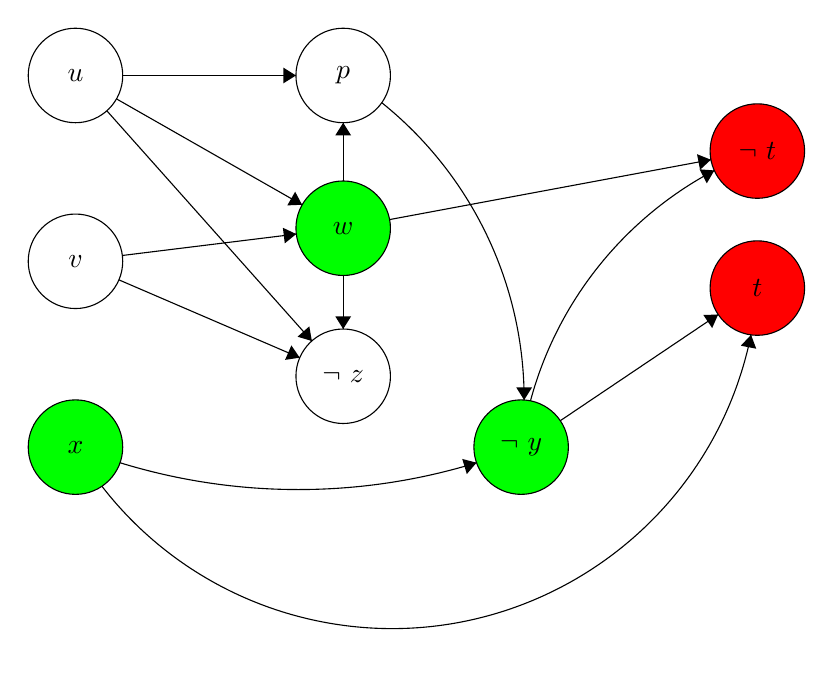
\begin{tikzpicture}[scale=0.2]
\tikzstyle{every node}+=[inner sep=0pt]
\draw [black] (10.2,-9.8) circle (3);
\draw (10.2,-9.8) node {$u$};
\draw [black] (10.2,-21.6) circle (3);
\draw (10.2,-21.6) node {$v$};
\draw [black,fill=green] (10.2,-33.4) circle (3);
\draw (10.2,-33.4) node {$x$};
\draw [black,fill=green] (27.2,-19.5) circle (3);
\draw (27.2,-19.5) node {$w$};
\draw [black] (27.2,-28.9) circle (3);
\draw (27.2,-28.9) node {$\neg\mbox{ }z$};
\draw [black] (27.2,-9.8) circle (3);
\draw (27.2,-9.8) node {$p$};
\draw [black,fill=green] (38.5,-33.4) circle (3);
\draw (38.5,-33.4) node {$\neg\mbox{ }y$};
\draw [black,fill=red] (53.5,-23.3) circle (3);
\draw (53.5,-23.3) node {$t$};
\draw [black,fill=red] (53.5,-14.6) circle (3);
\draw (53.5,-14.6) node {$\neg\mbox{ }t$};
\draw [black] (13.2,-9.8) -- (24.2,-9.8);
\fill [black] (24.2,-9.8) -- (23.4,-9.3) -- (23.4,-10.3);
\draw [black] (12.81,-11.29) -- (24.59,-18.01);
\fill [black] (24.59,-18.01) -- (24.15,-17.18) -- (23.65,-18.05);
\draw [black] (12.19,-12.04) -- (25.21,-26.66);
\fill [black] (25.21,-26.66) -- (25.05,-25.73) -- (24.3,-26.39);
\draw [black] (12.96,-22.78) -- (24.44,-27.72);
\fill [black] (24.44,-27.72) -- (23.91,-26.94) -- (23.51,-27.86);
\draw [black] (27.2,-16.5) -- (27.2,-12.8);
\fill [black] (27.2,-12.8) -- (26.7,-13.6) -- (27.7,-13.6);
\draw [black] (35.67,-34.393) arc (-72.89572:-107.10428:38.489);
\fill [black] (35.67,-34.39) -- (34.76,-34.15) -- (35.05,-35.11);
\draw [black] (53.095,-26.27) arc (-11.45045:-142.28988:23.271);
\fill [black] (53.1,-26.27) -- (52.45,-26.96) -- (53.43,-27.15);
\draw [black] (40.99,-31.72) -- (51.01,-24.98);
\fill [black] (51.01,-24.98) -- (50.07,-25.01) -- (50.63,-25.84);
\draw [black] (39.093,-30.461) arc (164.92322:117.90598:23.461);
\fill [black] (50.77,-15.83) -- (49.83,-15.76) -- (50.29,-16.65);
\draw [black] (29.65,-11.528) arc (51.25675:-0.08528:24.161);
\fill [black] (38.69,-30.41) -- (39.19,-29.61) -- (38.19,-29.61);
\draw [black] (27.2,-22.5) -- (27.2,-25.9);
\fill [black] (27.2,-25.9) -- (27.7,-25.1) -- (26.7,-25.1);
\draw [black] (30.15,-18.95) -- (50.55,-15.15);
\fill [black] (50.55,-15.15) -- (49.67,-14.8) -- (49.86,-15.79);
\draw [black] (13.18,-21.23) -- (24.22,-19.87);
\fill [black] (24.22,-19.87) -- (23.37,-19.47) -- (23.49,-20.46);
\end{tikzpicture}
\end{center}
Der Schnitt würde direkt an den beiden roten Knoten entlang verlaufen wenn man ihn einzeichnen sollte. Hier die 1UIP Klausel: 
\begin{center}
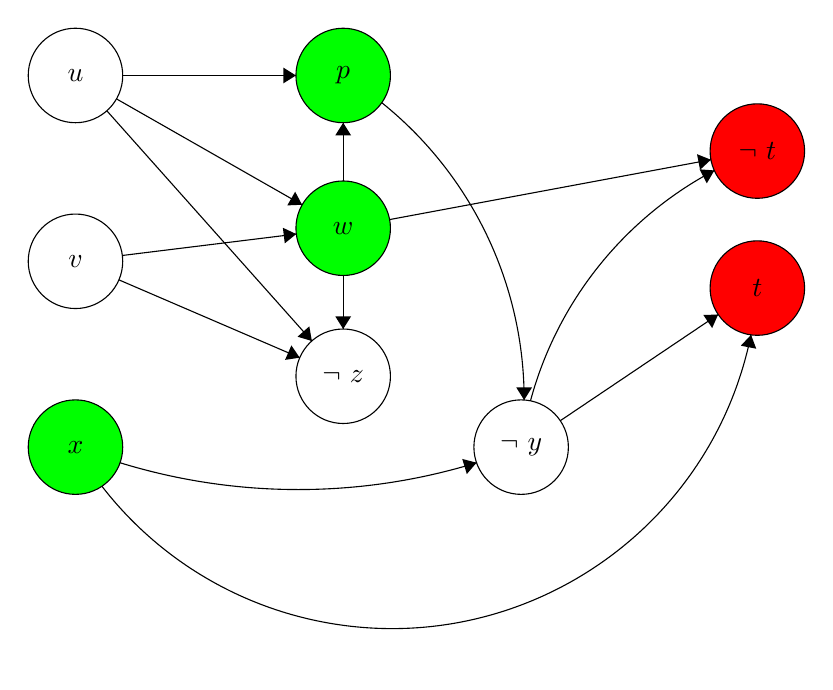
\begin{tikzpicture}[scale=0.2]
\tikzstyle{every node}+=[inner sep=0pt]
\draw [black] (10.2,-9.8) circle (3);
\draw (10.2,-9.8) node {$u$};
\draw [black] (10.2,-21.6) circle (3);
\draw (10.2,-21.6) node {$v$};
\draw [black,fill=green] (10.2,-33.4) circle (3);
\draw (10.2,-33.4) node {$x$};
\draw [black,fill=green] (27.2,-19.5) circle (3);
\draw (27.2,-19.5) node {$w$};
\draw [black] (27.2,-28.9) circle (3);
\draw (27.2,-28.9) node {$\neg\mbox{ }z$};
\draw [black,fill=green] (27.2,-9.8) circle (3);
\draw (27.2,-9.8) node {$p$};
\draw [black] (38.5,-33.4) circle (3);
\draw (38.5,-33.4) node {$\neg\mbox{ }y$};
\draw [black,fill=red] (53.5,-23.3) circle (3);
\draw (53.5,-23.3) node {$t$};
\draw [black,fill=red] (53.5,-14.6) circle (3);
\draw (53.5,-14.6) node {$\neg\mbox{ }t$};
\draw [black] (13.2,-9.8) -- (24.2,-9.8);
\fill [black] (24.2,-9.8) -- (23.4,-9.3) -- (23.4,-10.3);
\draw [black] (12.81,-11.29) -- (24.59,-18.01);
\fill [black] (24.59,-18.01) -- (24.15,-17.18) -- (23.65,-18.05);
\draw [black] (12.19,-12.04) -- (25.21,-26.66);
\fill [black] (25.21,-26.66) -- (25.05,-25.73) -- (24.3,-26.39);
\draw [black] (12.96,-22.78) -- (24.44,-27.72);
\fill [black] (24.44,-27.72) -- (23.91,-26.94) -- (23.51,-27.86);
\draw [black] (27.2,-16.5) -- (27.2,-12.8);
\fill [black] (27.2,-12.8) -- (26.7,-13.6) -- (27.7,-13.6);
\draw [black] (35.67,-34.393) arc (-72.89572:-107.10428:38.489);
\fill [black] (35.67,-34.39) -- (34.76,-34.15) -- (35.05,-35.11);
\draw [black] (53.095,-26.27) arc (-11.45045:-142.28988:23.271);
\fill [black] (53.1,-26.27) -- (52.45,-26.96) -- (53.43,-27.15);
\draw [black] (40.99,-31.72) -- (51.01,-24.98);
\fill [black] (51.01,-24.98) -- (50.07,-25.01) -- (50.63,-25.84);
\draw [black] (39.093,-30.461) arc (164.92322:117.90598:23.461);
\fill [black] (50.77,-15.83) -- (49.83,-15.76) -- (50.29,-16.65);
\draw [black] (29.65,-11.528) arc (51.25675:-0.08528:24.161);
\fill [black] (38.69,-30.41) -- (39.19,-29.61) -- (38.19,-29.61);
\draw [black] (27.2,-22.5) -- (27.2,-25.9);
\fill [black] (27.2,-25.9) -- (27.7,-25.1) -- (26.7,-25.1);
\draw [black] (30.15,-18.95) -- (50.55,-15.15);
\fill [black] (50.55,-15.15) -- (49.67,-14.8) -- (49.86,-15.79);
\draw [black] (13.18,-21.23) -- (24.22,-19.87);
\fill [black] (24.22,-19.87) -- (23.37,-19.47) -- (23.49,-20.46);
\end{tikzpicture}
\end{center}
Der Schnitt würde vertikal zwischen den Knoten $\neg z$ und $\neg y$ verlaufen. Schlussendlich noch die Decision Clause eingezeichnet:
\begin{center}
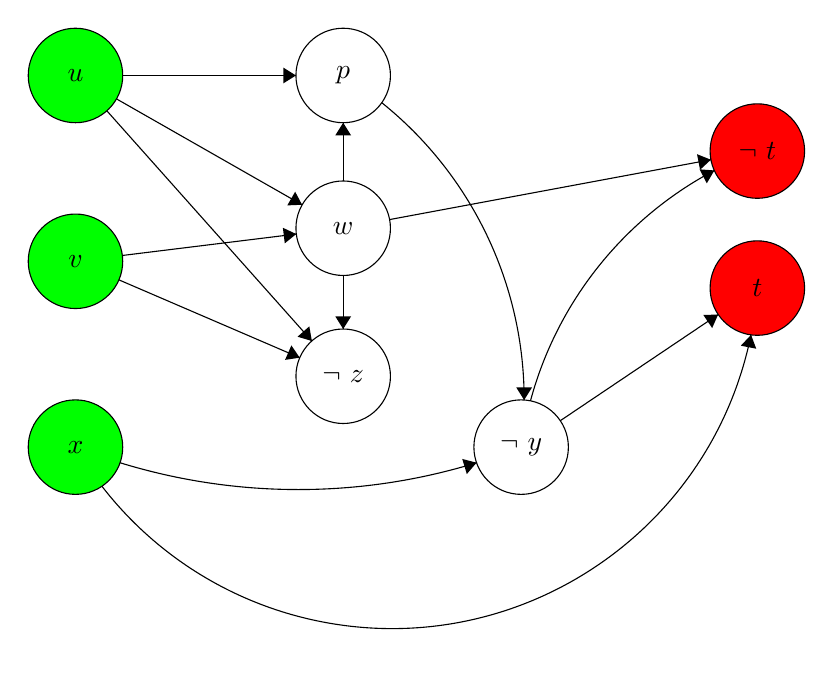
\begin{tikzpicture}[scale=0.2]
\tikzstyle{every node}+=[inner sep=0pt]
\draw [black,fill=green] (10.2,-9.8) circle (3);
\draw (10.2,-9.8) node {$u$};
\draw [black,fill=green] (10.2,-21.6) circle (3);
\draw (10.2,-21.6) node {$v$};
\draw [black,fill=green] (10.2,-33.4) circle (3);
\draw (10.2,-33.4) node {$x$};
\draw [black] (27.2,-19.5) circle (3);
\draw (27.2,-19.5) node {$w$};
\draw [black] (27.2,-28.9) circle (3);
\draw (27.2,-28.9) node {$\neg\mbox{ }z$};
\draw [black] (27.2,-9.8) circle (3);
\draw (27.2,-9.8) node {$p$};
\draw [black] (38.5,-33.4) circle (3);
\draw (38.5,-33.4) node {$\neg\mbox{ }y$};
\draw [black,fill=red] (53.5,-23.3) circle (3);
\draw (53.5,-23.3) node {$t$};
\draw [black,fill=red] (53.5,-14.6) circle (3);
\draw (53.5,-14.6) node {$\neg\mbox{ }t$};
\draw [black] (13.2,-9.8) -- (24.2,-9.8);
\fill [black] (24.2,-9.8) -- (23.4,-9.3) -- (23.4,-10.3);
\draw [black] (12.81,-11.29) -- (24.59,-18.01);
\fill [black] (24.59,-18.01) -- (24.15,-17.18) -- (23.65,-18.05);
\draw [black] (12.19,-12.04) -- (25.21,-26.66);
\fill [black] (25.21,-26.66) -- (25.05,-25.73) -- (24.3,-26.39);
\draw [black] (12.96,-22.78) -- (24.44,-27.72);
\fill [black] (24.44,-27.72) -- (23.91,-26.94) -- (23.51,-27.86);
\draw [black] (27.2,-16.5) -- (27.2,-12.8);
\fill [black] (27.2,-12.8) -- (26.7,-13.6) -- (27.7,-13.6);
\draw [black] (35.67,-34.393) arc (-72.89572:-107.10428:38.489);
\fill [black] (35.67,-34.39) -- (34.76,-34.15) -- (35.05,-35.11);
\draw [black] (53.095,-26.27) arc (-11.45045:-142.28988:23.271);
\fill [black] (53.1,-26.27) -- (52.45,-26.96) -- (53.43,-27.15);
\draw [black] (40.99,-31.72) -- (51.01,-24.98);
\fill [black] (51.01,-24.98) -- (50.07,-25.01) -- (50.63,-25.84);
\draw [black] (39.093,-30.461) arc (164.92322:117.90598:23.461);
\fill [black] (50.77,-15.83) -- (49.83,-15.76) -- (50.29,-16.65);
\draw [black] (29.65,-11.528) arc (51.25675:-0.08528:24.161);
\fill [black] (38.69,-30.41) -- (39.19,-29.61) -- (38.19,-29.61);
\draw [black] (27.2,-22.5) -- (27.2,-25.9);
\fill [black] (27.2,-25.9) -- (27.7,-25.1) -- (26.7,-25.1);
\draw [black] (30.15,-18.95) -- (50.55,-15.15);
\fill [black] (50.55,-15.15) -- (49.67,-14.8) -- (49.86,-15.79);
\draw [black] (13.18,-21.23) -- (24.22,-19.87);
\fill [black] (24.22,-19.87) -- (23.37,-19.47) -- (23.49,-20.46);
\end{tikzpicture}
\end{center}
Der Schnitt würde vertikal rechts von den Knoten u, v und x verlaufen.
\end{enumerate}



\noindent\textbf{Aufgabe 3.2}\\\smallskip
Im folgenden der Verlauf des Algorithmus bis zum ersten Konflikt. Die einzelnen Zeilen kommen entweder durch Entscheidung einer Belegung oder UP zustande. Die Reihenfolge der Variablen und die Belegung mit wahr im Entscheidungsfall ist wie auf dem Blatt verlangt umgesetzt.
\begin{center}
\begin{tabular}{|c|c|c|c|}
\hline 
\rule[-1ex]{0pt}{2.5ex} Level & Variable & Wert & Grund \\ 
\hline 
\rule[-1ex]{0pt}{2.5ex} 1 & a & $\top$ & Decision \\ 
\hline 
\rule[-1ex]{0pt}{2.5ex}  & b & $\top$ & $\{\neg a, b\}$ \\ 
\hline 
\rule[-1ex]{0pt}{2.5ex}  & w & $\bot$ & $\{\neg a, \neg b, \neg w\}$ \\ 
\hline 
\rule[-1ex]{0pt}{2.5ex} 2 & z & $\top$ & Decision \\ 
\hline 
\rule[-1ex]{0pt}{2.5ex}  & x & $\top$ & $\{\neg a, \neg b, w, \neg z, x\}$ \\ 
\hline 
\rule[-1ex]{0pt}{2.5ex}  & x & $\bot$ & $\{\neg a, \neg b, w, \neg z, \neg x\}$ \\ 
\hline 
\end{tabular} 
\end{center}

Der erste Konflikt, x muss wegen $\{\neg a, \neg b, w, \neg z, x\}$ auf wahr und wegen $\{\neg a, \neg b, w, \neg z, \neg x\}$ auf falsch gesetzt werden. Berechne aus beiden die Resolvente $\{\neg a, \neg b, w, \neg z\}$. Diese ist bereits 1UIP, da mit z nur eine Variable von Level 2 vorkommt und Level 2 das höchste vorkommende Level ist. Füge also die Klausel $\{\neg a, \neg b, w, \neg z\}$ zur Formel hinzu, lösche alle Belegungen bis inklusive Level 2 und die Unit-Klausel zwingt im nächsten Schritt z dazu mit falsch belegt zu werden. z ist also keine Entscheidungsvariable mehr sondern wurde durch UP belegt. Im folgenden der Verlauf des Algorithmus bis zum zweiten Konflikt:
\begin{center}
\begin{tabular}{|c|c|c|c|}
\hline 
\rule[-1ex]{0pt}{2.5ex} Level & Variable & Wert & Grund \\ 
\hline 
\rule[-1ex]{0pt}{2.5ex} 1 & a & $\top$ & Decision \\ 
\hline 
\rule[-1ex]{0pt}{2.5ex}  & b & $\top$ & $\{\neg a, b\}$ \\ 
\hline 
\rule[-1ex]{0pt}{2.5ex}  & w & $\bot$ & $\{\neg a, \neg b, \neg w\}$ \\ 
\hline 
\rule[-1ex]{0pt}{2.5ex}  & z & $\bot$ & $\{\neg a, \neg b, w, \neg z\}$ \\ 
\hline 
\rule[-1ex]{0pt}{2.5ex}  & y & $\top$ & $\{\neg a, \neg b, w, z, y\}$ \\ 
\hline 
\rule[-1ex]{0pt}{2.5ex}  & y & $\bot$ & $\{\neg a, \neg b, w, z, \neg y\}$ \\ 
\hline 
\end{tabular} 
\end{center}
Der zweite Konflikt, y muss wegen $\{\neg a, \neg b, w, z, y\}$ auf wahr und wegen $\{\neg a, \neg b, w, z, \neg y\}$ auf falsch gesetzt werden. Berechne sukzessiv die Resolvente, bis eine 1UIP-Klausel entsteht:
\begin{align*}
\{\neg a, \neg b, w, z\} & = (\{\neg a, \neg b, w, z, y\} \setminus \{y\}) \cup (\{\{\neg a, \neg b, w, z, \neg y\}\} \setminus \{\neg y\}) \\
\{\neg a, \neg b, w\} & = (\{\neg a, \neg b, w, z\} \setminus \{z\}) \cup (\{\neg a, \neg b, w, \neg z\} \setminus \{\neg z\}) \\
\{\neg a, \neg b\} & = (\{\neg a, \neg b, w\} \setminus \{w\}) \cup (\{\neg a, \neg b, \neg w\} \setminus \{\neg w\}) \\
\{\neg a\} & = (\{\neg a, \neg b\} \setminus \{\neg b\}) \cup (\{\neg a, b\} \setminus \{b\})
\end{align*}
$\{\neg a\}$ ist die 1UIP-Klausel und a hat Level 1, entferne also die Belegung aller Variablen auf Level 1 und füge die Klausel $\{\neg a\}$ zur Formel hinzu. Im nächsten Schritt wird a also durch UP auf falsch gesetzt. Der weitere Verlauf des Algorithmus:
\begin{center}
\begin{tabular}{|c|c|c|c|}
\hline 
\rule[-1ex]{0pt}{2.5ex} Level & Variable & Wert & Grund \\ 
\hline 
\rule[-1ex]{0pt}{2.5ex} 0 & a & $\bot$ & $\{\neg a\}$ \\ 
\hline 
\rule[-1ex]{0pt}{2.5ex}  & b & $\top$ & Decision \\ 
\hline 
\rule[-1ex]{0pt}{2.5ex}  & w & $\bot$ & $\{a, \neg b, \neg w\}$ \\ 
\hline 
\rule[-1ex]{0pt}{2.5ex}  & x & $\top$ & $\{a, \neg b, w, \neg x\}$ \\ 
\hline 
\end{tabular} 
\end{center}
Es sind keine unerfüllten Klauseln mehr übrig, also ist eine erfüllende Belegung gefunden. Die Belegungen für y und z sind egal, da ein Literal pro Klausel schon erfüllt ist durch die Belegung von a, b, w und x. Also ist eine mögliche erfüllende Belegung $\alpha = \{a \mapsto 0, b \mapsto 1, w \mapsto 0, x \mapsto 1, y \mapsto 0, z \mapsto 0\}$.


\noindent\textbf{Aufgabe 3.3}\\\smallskip
\begin{enumerate}
\item Sei $C \in \phi$ beliebig. Es gilt trivialerweise, dass $(\exists l \in \emptyset: \overline{l} \in C)$ falsch ist, da jede Existenzaussage über die leere Menge falsch ist. Damit ist die Implikation $(\exists l \in \emptyset: \overline{l} \in C) \Rightarrow A \cap C \neq \emptyset$ wahr. Da C beliebig war gilt die Aussage für alle $C \in \phi$. Die andere Bedingung für Autarkien, $l \in \emptyset \Rightarrow \overline{l} \notin \emptyset$ gilt ebenfalls trivialerweise, da dies eine implizite Allaussage ist und Allaussagen über die leere Menge immer wahr sind. Damit ist $\emptyset$ per Definition eine Autarkie.

\item Die Definition von Autarkien auf dem Übungsblatt setzt nicht voraus, dass die Literale aus $A$ wirklich in $\phi$ vorkommen müssen, also kann leicht ein Gegenbeispiel angeben werden: $\phi = \{\{x, y\}\}, A = \{\neg x, y\}$, dann enthält die einzige Klausel von $\phi$ ein komplementäres Literal zu einem Literal in $A$ und $A \cap \{x, y\} = \{y\} \neq \emptyset$, außerdem enthält A keine komplementären Literale, also ist A eine Autarkie. x ist außerdem pure in dieser Formel, da x nur unnegiert vorkommt. Aber $A \cup \{x\}$ ist keine Autarkie, weil die erste Bedingung in der Definition verbietet, dass komplementäre Literale in einer Autarkie enthalten sind. Also ist die Aussage falsch.

\item Betrachte das folgende Beispiel: $\phi = \{\{x, y\}, \{\neg x, y\}\}, A = \{\neg x, y\}$, A ist aus dem selben Grund wie in der letzten Teilaufgabe eine Autarkie, die zweite Klausel enthält kein komplementäres Literal zu einem Literal aus A und muss desshalb nicht betrachtet werden. Die Belegung, die x auf wahr setzt und y auf wahr setzt erfüllt $\phi$. Allerdings wird $\phi \cup \bigcup_{l \in A}\{\{l\}\}$ von dieser Belegung nicht erfüllt, da $\{\neg x\}$ offenbar nicht erfüllt wird. Also sind die Formeln nicht semantisch Äquivalent, die Aussage ist nicht allgemein wahr. 

\item Die Aussage ist wahr. Alle Klauseln, die ein komplementäres Literal zu einem Literal aus A enthalten, enthalten per Definition von Autarkien ebenfalls ein Literal aus A. Die neuen Klauseln werden durch UP alle erfüllt, da keine komplementären Literale in A enthalten sein können, und alle Klauseln, die ein komplementäres Literal zu einem Literal aus A enthalten,  werden auch erfüllt, da diese Klauseln wie schon gesagt ebenfalls ein Literal aus A enthalten das jetzt durch die Unit-Klauseln erfüllt werden muss. Mit dieser Überlegung folgt nun: war $\phi$ erfüllbar ist nun auch die neue Formel erfüllbar, da alle Klauseln, die von der Autarkie betroffen sind, erfüllt werden durch die Belegung, die durch UP erzwungen wird, und die Klauseln, in denen kein komplementäres Literal zu einem Literal in A vorkommt, entweder ebenfalls durch diese Belegung erfüllt werden (falls sie ein Literal aus A enthalten) oder durch die Belegung der Variablen, die diese Klauseln in einer erfüllenden Belegung für $\phi$ erfüllen. In letzterem Fall enthalten die betroffenen Klauseln nur Literale die weder komplementiert noch normal in A vorkommen, also Widerspricht eine Belegung die $\phi$ erfüllt auf die Variablen in diesen Klauseln eingeschränkt nicht der Belegung, die durch UP erzwungen wurde. Kombiniert man also die beiden genannten Belegungen erfüllt sie die neue Formel und die neue Formel ist damit erfüllbar. War $\phi$ nicht erfüllbar ist offenbar die neue Formel auch nicht erfüllbar, da durch neue Klauseln eine unerfüllbare Formel in CNF ganz allgemein nicht erfüllbar werden kann, da es immer noch keine Belegung gibt die alle 'alten' Klauseln erfüllt.

\item Die Ausgabenstellung verlangt nicht, dass $\phi$ erfüllbar ist. Betrachte $\phi = \{\{x\}, \{\neg x\}, \{y\}, \{\neg y\}\}$. Sowohl $\{\{x\}, \{\neg x\}\}$ als auch $\{\{y\},\{\neg y\}\}$ sind jeweils ein MUS bezüglich $\phi$, da jeweils alle drei echten Teilmengen offensichtlich erfüllbar sind, aber $\{\{x\}, \{\neg x\}\} \neq \{\{y\}, \{\neg y\}\}$, also muss ein MUS nicht eindeutig sein. Damit ist die Aussage im allgemeinen nicht wahr.

\item Die Behauptung ist wahr. Sei M ein beliebiges MUS von $\phi$. Angenommen es gäbe eine Autarkie A, sodass es eine Klausel $C \in M$ gibt mit $A \cap C \neq \emptyset$. Wähle $l \in A \cap C$ beliebig, da der Schnitt nicht leer ist muss ein solches Literal existieren. Entferne nun alle Klauseln aus M, die $l$ enthalten, also mindestens eine. Sei M' die Klauselmenge, die so entsteht. Da A eine Autarkie von $\phi$ ist, ist $A$ auch eine Autarkie von M, da sich die Definition von Autarkien nur auf einzelne Klauseln bezieht, das selbe gilt für M'. Damit ist $M' \cup \bigcup_{l' \in A} \{\{l'\}\}$ erfüllbarkeits-äquivalent zu $M'$ (folgt aus vorheriger Teilaufgabe) und eine erfüllende Belegung von $M'$ muss offenbar $l$ auf wahr setzen, da die Unit-Clause $\{l\}$ enthalten ist. Da $M' \subsetneq M$ folgt aus der Definition eines MUS, dass $M'$ erfüllbar ist. Also ist auch $M'  \cup \bigcup_{l' \in A} \{\{l'\}\}$ erfüllbar und jede erfüllende Belegung setzt das Literal l auf wahr. Diese Belegung erfüllt nun auch die Klauseln, die aus M entfernt wurden um M' zu erhalten, da diese $l$ enthalten haben, erfüllt damit also alle Klauseln in $M$. Widerspruch, $M$ ist ein MUS und damit unerfüllbar. Also gibt es keine Autarkie, welche die Bedingung der Aufgabenstellung verletzt. Da M ein beliebiges MUS ist gilt die Behauptung für alle MUS und alle Autarkien von $\phi$.
\end{enumerate}
\end{document}
